\section{Исследовательская часть}

\subsection{Технические характеристики}
Технические характеристики устройства, на котором выполнялось исследование:
\begin{itemize}
	\item операционная система: Ubuntu 22.04, 64-bit;
	\item оперативная память: 8 Гб;
	\item процессор: AMD Ryzen5 4500U \cite{proc}.
\end{itemize}

\subsection{Исследование генерируемых систем}
При разработке программы для генерации экспертных систем и добавления их в базу данных было обнаружено, что гауссова функция распределения и $\Pi$-функция, используемая на уровне БД, имеют существенные отличия, влияющие на результат работы нечеткой экспертной системы. 

На рисунке \ref{fig:a-b} а) приведены сгенерированные программно гауссовы \\*функции принадлежности для одной из входных переменных системы, \ref{fig:c-else} в) -- адаптированные под хранение в базе данных. Для сглаживания различий принято решение сохранять в базу гауссовы функции в виде $\Pi$-функций, вычисляемых по формуле \ref{eq:P-func}, с параметрами $\beta = \mu$, $\gamma = 3 \cdot \sigma$, где $\mu$ -- математическое ожидание функции плотности нормального распределения, $\sigma$ -- среднеквадратическое отклонение. 

\begin{figure}[H]
	\begin{minipage}[h]{0.49\linewidth}
		\centering
		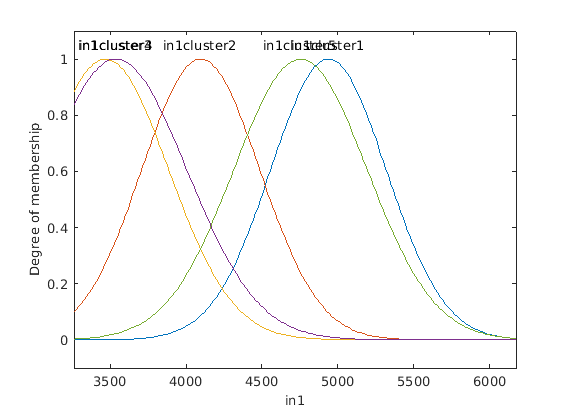
\includegraphics[width=1\linewidth]{img/gauss}
		a)\\
	\end{minipage}
	\hfill
	\begin{minipage}[h]{0.49\linewidth}
		\centering
		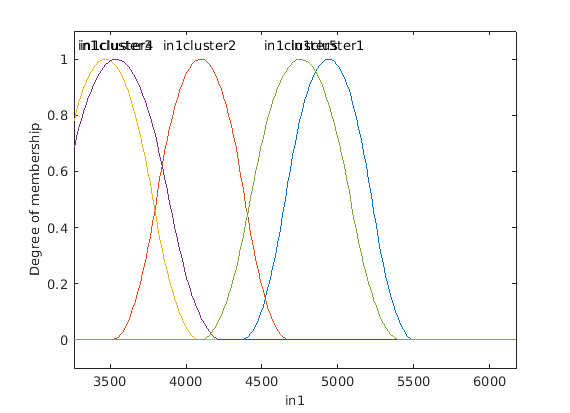
\includegraphics[width=1\linewidth]{img/1_5sigma}
		б)\\
	\end{minipage}
	\caption{Графики функций принадлежности переменной: а) сгенерированные с помощью matlab, б) $\Pi$-функции с параметрами $\gamma=1.5\cdot\sigma$}
	\label{fig:a-b}
\end{figure}
\begin{figure}[H]
	\begin{minipage}[h]{0.49\linewidth}
		\centering
		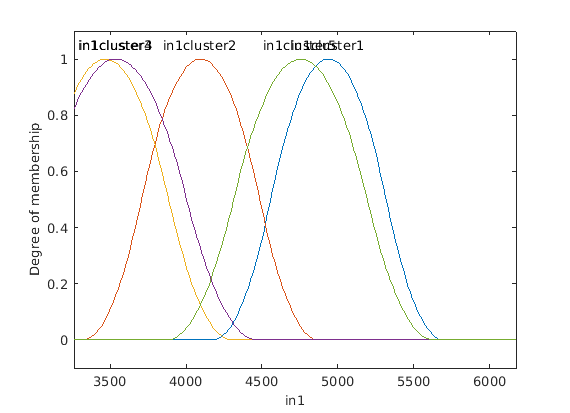
\includegraphics[width=1\linewidth]{img/2sigma}
		а)\\
	\end{minipage}
	\hfill
	\begin{minipage}[h]{0.49\linewidth}
		\centering
		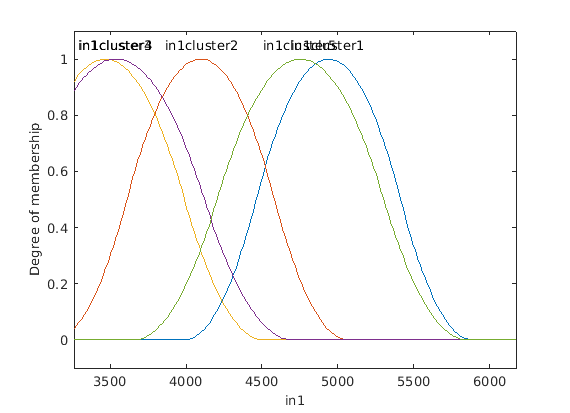
\includegraphics[width=1\linewidth]{img/2_5sigma}
		б)\\	
	\end{minipage}
	\vfill
	\begin{minipage}[h]{0.49\linewidth}
		\centering
		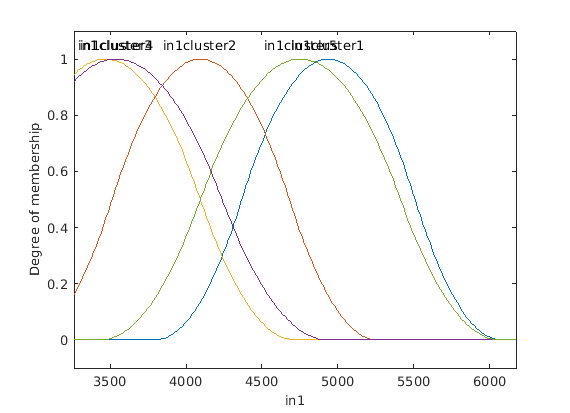
\includegraphics[width=1\linewidth]{img/3sigma}
		в)\\
	\end{minipage}
	\hfill
	\begin{minipage}[h]{0.49\linewidth}
		\centering
		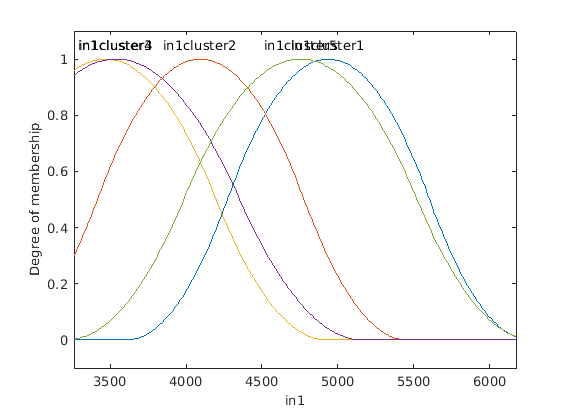
\includegraphics[width=1\linewidth]{img/3_5sigma}
		г)\\
	\end{minipage}
	\vfill
	\begin{minipage}[h]{0.49\linewidth}
		\centering
		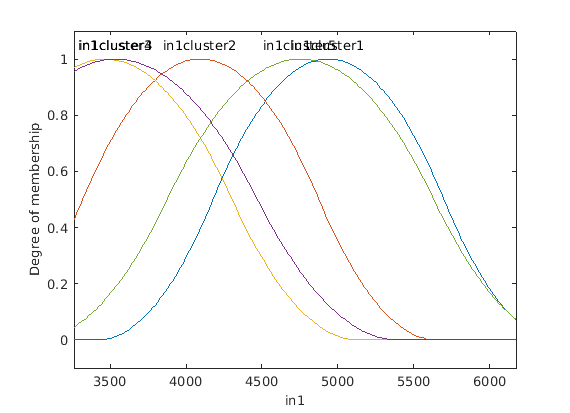
\includegraphics[width=1\linewidth]{img/4sigma}
		д)
	\end{minipage}

	\caption{Графики функций принадлежности переменной: а) $\Pi$-функции с параметрами $\gamma=2\cdot\sigma$, б) $\Pi$-функции с параметрами $\gamma=2.5\cdot\sigma$, в) $\Pi$-функции с параметрами $\gamma=3\cdot\sigma$, г) $\Pi$-функции с параметрами $\gamma=3.5\cdot\sigma$, д) $\Pi$-функции с параметрами $\gamma=4\cdot\sigma$}
	\label{fig:c-else}
\end{figure}

При меньшем коэффициенте для вычисления $\gamma$ и количестве кластеров, меньшем четырех, возможно появление больших зон, в которых все функции принадлежности для переменной равны 0 (рисунок \ref{fig:a-b} б), рисунок \ref{fig:c-else} а) -- б)), что не позволяет получить корректный результат работы системы. 

Большее значение коэффициента создает существенные отличия в интервале значений, в которых значение функции принадлежности больше 0, поскольку, согласно правилу трех сигм для нормального распределения, 99.7\% значений лежат в пределах трех стандартных отклонений от математического ожидания. Примеры $\Pi$-функций принадлежности при $\gamma = 3.5 \cdot \sigma$ и $\gamma = 4 \cdot \sigma$ представлен на рисунке \ref{fig:c-else} г)--д).

В результате подобных изменений также меняются значения, получаемые при нечетком выводе. Из-за неполного соответствия интервалов, в которых функции принадлежности принимают значения, большие 0, возможны ситуации при которых невозможно получить результат логического вывода, если все правила системы конъюнктивные и хотя бы 1 антецедент в каждом из них принимает значение, равное 0, следовательно, ни одно из правил невозможно активизировать. В связи с этим в дальнейшем возникает необходимость добавления поддержки чистых гауссовых функций, а не их аппроксимации в виде $\Pi$-функций, на уровне базы данных.

В таблице \ref{tab:tests} приведено сравнение результатов работы системы с одной выходной переменной и 5 кластерами при разных коэффициентах $c$ для $\Pi$-функции ($\gamma = c \cdot \sigma$) с исходными данными и значением, вычисленным с использованием средств Matlab и исходных гауссовых функций на основе набора данных, приведенного в листинге \ref{lst:inout}. Значение, равное 0, говорит о том, что ни одно из правил системы не было активизировано и получить результат не удалось. Использованные наборы значений:

\begin{enumerate}
	\item in1 = 3356.09, in2 = 6509.38, in3 = 5587.47, in4 = 4106.31, in5 = 5512.47
	\item in1 = 4915.10, in2 = 6460.23, in3 = 6069.10, in4 = 4309.56, in5 = 5699.36
\end{enumerate} 

\begin{lstlisting}[caption=Пример входных и выходных данных для генерации нечеткой экспертной системы (последний столбец - значения выходной переменной), label={lst:inout}]
6173.82    6051.42    5164.89    2395.29    6173.63    4070.99 
3262.04    6290.51    5795.75    2546.39    6170.57    4826.16 
4021.02    6654.06    6350.57    2402.60    4601.78    5653.51 
3440.28    6655.82    4615.67    3789.04    4547.42    4230.85 
4369.20    6419.66    4095.09    4157.41    4917.27    5623.29 
4915.10    6460.23    6069.10    4309.56    5699.36    6924.39 
3400.89    6695.89    7003.25    2476.91    6074.97    4165.13 
4942.51    6759.04    4182.98    4479.01    5744.79    5589.45 
\end{lstlisting}

\begin{table}[H]
		\captionsetup{justification=raggedright, singlelinecheck=false}
	\caption[]{\label{tab:tests} Результаты работы системы}
	\begin{center}
		\begin{tabular}{|c|c|c|c|c|c|c|c|c|}
			\hline
			& $c=1.5$ & $c=2$ & $c=2.5$ & $c=3$ & $c=3.5$ & $c=4$ & Гаусс & Ожидание\\
			\hline
			1 & 0 & 0 & 0 & 4256.6 & 4579.4 & 4622.8 & 4921.3 & 4365.8 \\
			\hline
			2 & 5571.7 & 0 & 7629.6 & 7802 & 4792.9 & 8196.3 & 6361.3 & 6924.4 \\
			\hline
		\end{tabular}

	\end{center}
\end{table}

\subsection{Исследование времени работы запросов}
Получение результата работы системы при большом количестве правил может быть ресурсоемким, поэтому для оптимизации времени получения результата работы системы предлагается кэшировать полученные данные с помощью in-memory базы данных Redis на 5 минут, если пользователь не изменяет значения входных переменных. На рисунке \ref{fig:redis} приведена зависимость времени получения результата запроса для системы типа Мамдани с 5 входными, 4 выходными переменными и 7 правилами нечеткого вывода (соответственно, для каждой переменной создается 7 функций принадлежности) от номера итерации. Значение времени выполнения запроса для каждой итерации вычисляется путем усреднения времени выполнения 50 запросов. Для графика с использованием кэширования в Redis раз в 2 итерации происходит сброс кэширования для оценки затрат на загрузку данных при истечении TTL/изменении значений переменных. 

\begin{figure}[H]
	\centering
	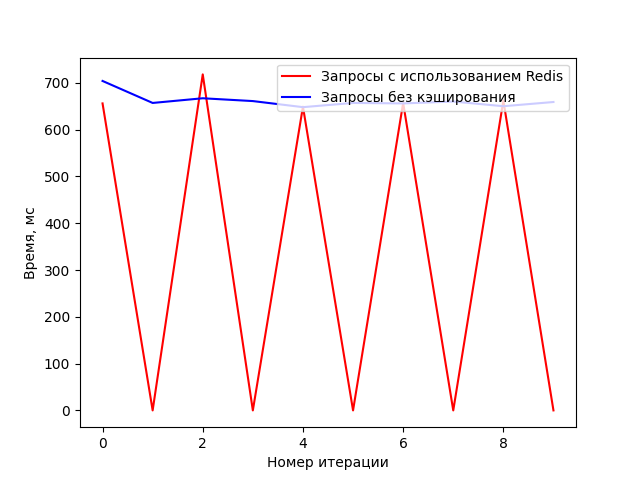
\includegraphics[width=0.7\linewidth]{img/redis}
	\caption{Исследование времени выполнения запросов с кэшированием и без}
	\label{fig:redis}
\end{figure}

На графике видно, что при использовании кэширования при отсутствии изменений значений переменных/функций принадлежности время выполнения запроса стремится к 0 миллисекундам, т.е. скорость увеличивается более чем в 600 раз. При необходимости обновления данных в кэше время выполнения запроса превышает время выполнения запроса без кэширования не более чем в 1,1 раз. Таким образом, использование встроенной базы данных для хранения результатов запросов оправдано, поскольку при хранении данных о 1000 экспертных системах время выполнения запроса для получения результата работы одной из них составляет около 0,6 секунд при небольшом количестве правил и функций принадлежности. При увеличении количества хранимых экспертных систем в 2 раза время выполнения запроса увеличивается в среднем в 1,15 раз (рисунок \ref{fig:timefromn}), кэширование результатов позволяет снизить нагрузку на базу данных и выполнение запроса.

\begin{figure}[H]
	\centering
	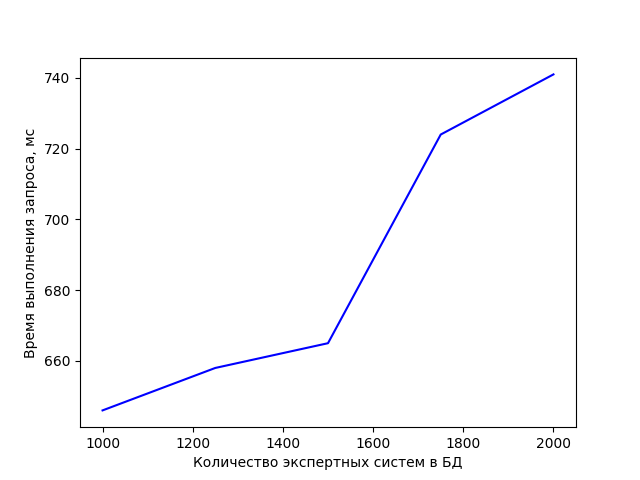
\includegraphics[width=0.7\linewidth]{img/time_from_n}
	\caption{Зависимость времени обработки запроса от количества экспертных систем в БД}
	\label{fig:timefromn}
\end{figure}

\subsection{Выводы}
В данном разделе проведено исследование корректности хранимых данных и получаемых результатов, выявлено, что $\Pi$-функция принадлежности не совпадает с гауссовой функцией, что ведет к изменению получаемых результатов работы нечеткой экспертной системы. 

Исследовано время выполнения запросов получения результата работы нечеткой экспертной системы с кэшированием во встроенной базе данных Redis и без. Выявлено, что кэширование результатов дает выигрыш более чем в 600 раз при повторном обращении, при первичном сохранении запрос выполняется не более чем в 1,1 раз дольше запроса без кэширования.

\pagebreak